\documentclass{standalone}
\usepackage{tikz}
\usepackage{ctex,siunitx}
\usepackage{tkz-euclide}
\usepackage{amsmath}
\usetikzlibrary{patterns, calc}
\usetikzlibrary {decorations.pathmorphing, decorations.pathreplacing, decorations.shapes,}
\begin{document}
\small
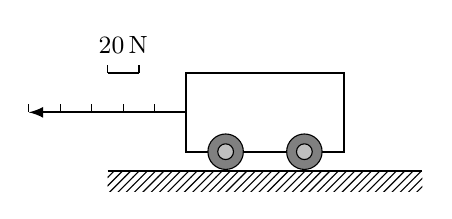
\begin{tikzpicture}[>=latex]
  \draw [semithick](0,0)rectangle (2,1);
  \fill [pattern = north east lines] (-1,-.5) rectangle (3,-.25);
  \draw [thick](-1,-.25)--(3,-.25);
  \draw [fill=gray](.5,0) circle (.225);
  \draw [fill=gray](1.5,0) circle (.225);
  \draw [fill=lightgray](.5,0) circle (.1);
  \draw [fill=lightgray](1.5,0) circle (.1);
  \draw [->, thick](0,0.5)--(-2,0.5);
  \foreach \i in {-.4,-.8,-1.2,-1.6,-2}
  {
      \draw[thin] (\i,0.6)--(\i,.5);
  }
  \draw[thin] (-1,1)--(-1,1.1);
  \draw[thin] (-0.6,1)--(-0.6,1.1);
  \draw[thin] (-1,1)--(-0.6,1);
  \node at (-0.8,1.35){\small \qty{20}{N}};
  \end{tikzpicture}
\end{document}